\subsubsection*{\S 交互设计的原则与目标}
\setcounter{problemname}{0}

\begin{problem}
	关于交互设计原则,以下描述正确的是:
	\uline{A}    
    %\vspace{-0.8em}
    %\begin{multicols}{2}
        \begin{enumerate}[label=\Alph*.]
            \item 设计应该使用用户容易理解的语言来表示错误信息
            \item 交互设计大师Donald Norman提出了十条启发式设计原则
            \item 在要求输入日期时为用户提供日历组件,这对应“用户应享有控制权和自主权”的设计原则
            \item 设计原则不能指导设计人员做出正确的决策
        \end{enumerate}
    %\end{multicols}
    %\vspace{-1em}
\end{problem}

\begin{solution}
A.正确,实际上界面上出现的一切信息都应该使用用户容易理解的语言。 B.启发式原则是由可用性工程之父Jacob Nielsen提出的。 C.提供日历组件是为了帮助用户避免错误。 D.设计原则是对前人的经验总结,能够帮助设计人员做出正确的决策。
\end{solution}


\begin{problem}
	以下哪一种情况不会在优秀产品中出现:
	\uline{C}    
    \vspace{-0.8em}
    \begin{multicols}{2}
        \begin{enumerate}[label=\Alph*.]
            \item 使用声音表达特定的含义
            \item 使用常用的快捷键,如``CTRL+Z"表示撤消
            \item 使用一长串命令来完成一个特定功能
            \item 图标们拥有清晰的语义
        \end{enumerate}
    \end{multicols}
    \vspace{-1em}
\end{problem}

\begin{solution}
C.一长串命令对用户而言既不容易记忆也不易于理解,交互中应使用简洁、清晰、用户易于理解的命令。
\end{solution}


\begin{problem}
	以下两个网页的主要区别在于:
	\uline{B}
\begin{figure}[H]
	\setcounter{subfigure}{0}
	\centering
	\vspace{-0.5em}	
	\subfloat{
	\begin{minipage}[t]{0.44\linewidth}
	\centering
	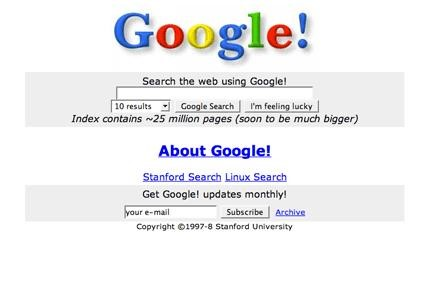
\includegraphics[width=0.97\linewidth]{2.3.1}
	\end{minipage}
	}
    \hfill
	\subfloat{
	\begin{minipage}[t]{0.5\linewidth}
	\centering
	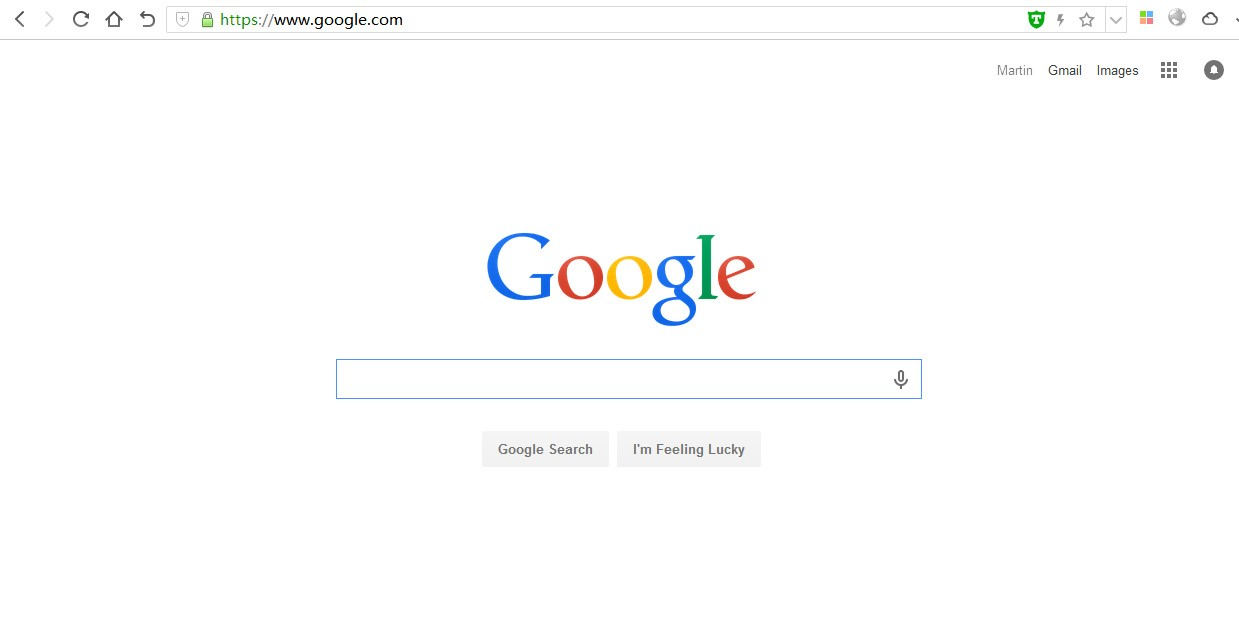
\includegraphics[width=0.97\linewidth]{2.3.2}
	\end{minipage}
	}
	\vspace{-1em}
\end{figure}
    \vspace{-0.8em}
    \begin{multicols}{2}
        \begin{enumerate}[label=\Alph*.]
            \item 第一个网站提供了对结果数量的控制
            \item 第二个网站只包含必要的UI组件
            \item 背景颜色
            \item 第二个网站的配色方案更优
        \end{enumerate}
    \end{multicols}
    \vspace{-1em}
\end{problem}

\begin{solution}
B.其他选项也都不同,但是最主要的区别还是下图去掉了很多多余的界面组件,使得“搜索框”这一系统入口变得更加明显。
\end{solution}


\begin{problem}
	提供加速器(如键盘快捷键等)的目的是为了提高系统的:
	\uline{D}    
    \vspace{-0.8em}
    \begin{multicols}{4}
        \begin{enumerate}[label=\Alph*.]
            \item 态度或喜爱程度
            \item 易学性
            \item 实用性
            \item 效率
        \end{enumerate}
    \end{multicols}
    \vspace{-1em}
\end{problem}

\begin{solution}
D.这一题比较简单,快捷键的主要特色是“快”。
\end{solution}


\begin{problem}
	能够帮助设计人员了解用户特定交互行为发生的原因的可用性工程方法是:
	\uline{A}    
    \vspace{-0.8em}
    \begin{multicols}{4}
        \begin{enumerate}[label=\Alph*.]
            \item 边做边说
            \item 用户和任务观察
            \item 启发式评估
            \item 场景
        \end{enumerate}
    \end{multicols}
    \vspace{-1em}
\end{problem}

\begin{solution}
A.边做边说是最有价值的单个可用性工程方法,简单的观察只能“知其然而不知其所以然”,通过让用户大声说出他们的想法,有助于明确用户遇到的具体问题。  B.该方法有助于了解用户的需要,通常用于早期需求获取阶段。  C.启发式评估的本质是专家模拟用户,性价比很高,但并不能替代对真实用户的观察和评估。  D.场景既可用于需求阶段,同人物角色一起描述需求;也可用于设计阶段,用于检验设计的细节。
\end{solution}